\documentclass[11pt]{article}

\usepackage[margin=1in]{geometry}
\usepackage{graphicx}
\usepackage{booktabs}
\usepackage{multirow}
\usepackage{amsmath}
\usepackage{amssymb}
\usepackage[numbers]{natbib}
\usepackage[hidelinks]{hyperref}
\usepackage{xcolor}

\graphicspath{{figures/}}
\setlength{\emergencystretch}{2em}

\title{Architecture-dependent effects of imbalance correction in melanoma classification: a controlled audit with fairness, calibration, and explanation analysis}

\author{
  Nursultan Zhanat$^{1,2}$ and Sun Baoshan$^{1,2,*}$\\[8pt]
  \parbox{0.92\textwidth}{\centering\small
  $^{1}$ School of Computer Science and Technology, Tiangong University, Tianjin 300387, China; sunbaoshan@tiangong.edu.cn (S.B.)\\
  $^{2}$ Tianjin Key Laboratory of Autonomous Intelligence Technology and Systems, Tiangong University, Tianjin 300387, China\\
  $^{*}$ Correspondence: sunbaoshan@tiangong.edu.cn; ORCID: 0000-0003-2193-3232
  }
}

\date{\today}

\begin{document}

\maketitle

\begin{abstract}
Melanoma classifiers are trained on imbalanced, predominantly light-skinned data. We ask whether imbalance correction changes CNN and transformer performance, whether calibration explains it, and how the models behave across skin tone and lesion contrast. We benchmark ResNet-50, EfficientNet-B0, and ViT-S/16 on HAM10000 under three pre-declared conditions: standard cross-entropy, focal loss with class-balanced sampling, and cross-entropy with strong augmentation. Each condition uses three seeds, a lesion-aware split, and a validation-selected threshold at 95\% specificity. Focal loss raises ViT-S/16 sensitivity by 8.2 points and lowers ResNet-50 by 11.7 and EfficientNet-B0 by 7.9. The direction is consistent, but every within-architecture interval includes zero. The EfficientNet-B0 versus ViT interaction is significant; the ResNet-50 versus ViT interaction is not. The AUC ordering is preserved, but the ViT closes the gap under focal loss, so the reversal is not purely a threshold effect. Calibration error rises 3.0x to 4.4x for the CNNs and 1.36x for the ViT, so calibration tracks the CNN loss, not the ViT gain. The dark stratum has a higher false positive rate at $L^*$ cutoffs of 55, 58, and 60, but the dark AUC differences are not significant at any cutoff. The false-negative $L^*$ association is significant for all three architectures; the false-positive association is significant only for ResNet-50. Grad-CAM mass is lower on darker images, but its error relationship differs by architecture. HIBA validation shows consistent CNN losses under focal loss, a seed-dependent ViT gain, and the best external performance under strong augmentation. This is a controlled audit.
\end{abstract}

\noindent\textbf{Keywords:} melanoma classification, class imbalance, fairness, calibration, explainable artificial intelligence, skin tone

\section{Introduction}

Melanoma is the most lethal form of skin cancer, and survival depends on early detection. Deep learning models have reached dermatologist-level accuracy on public dermoscopic benchmarks such as HAM10000 and the ISIC challenges \citep{tschandl2018ham10000,codella2018isic}. Three problems remain.

Public datasets are imbalanced. Benign lesions outnumber melanomas by roughly ten to one, and a classifier that predicts the majority class can look accurate while missing cancers. Focal loss and class-balanced sampling are common remedies \citep{lin2017focal}, but their effect is often reported for one architecture and one dataset.

The datasets are also skewed toward lighter skin. Fitzpatrick skin types V and VI are rare in public dermoscopic data, and models trained on lighter skin can lose sensitivity on darker skin \citep{groh2021fitzpatrick17k,daneshjou2022ddi,ruga2026pipsqueak}. The data needed to measure the gap are themselves scarce.

Deep models are opaque as well. Gradient-based attribution methods such as Grad-CAM and Integrated Gradients can show which pixels drive a prediction \citep{selvaraju2017gradcam,sundararajan2017ig}, but most dermatology papers use them as illustrations. They are rarely turned into quantitative measurements that can be tested across skin tone groups.

Most studies examine one of these problems at a time. Architecture comparisons often apply a single imbalance correction without checking whether it is neutral across architectures, and fairness studies report group-level performance without connecting it to attribution behaviour. This study connects the three in one benchmark.

We study HAM10000 \citep{tschandl2018ham10000} with a binary melanoma endpoint and three architectures: ResNet-50, EfficientNet-B0, and ViT-S/16. We use a lesion-aware split, three seeds per condition, and a validation-selected threshold at 95\% specificity. The test set is touched once per run.

Our contributions are:

\begin{enumerate}
  \item A controlled benchmark of three architectures under three pre-declared conditions: CE baseline, focal loss with class-balanced sampling, and CE with strong augmentation.
  \item Evidence that focal loss with class-balanced sampling improves ViT-S/16 but reduces the sensitivity of both CNNs, which reverses the point-estimate ranking at 95\% specificity. The paired within-architecture intervals include zero, while the difference-in-differences between each CNN and the ViT excludes zero. The AUC ranking is stable.
  \item A calibration analysis that shows focal loss with class-balanced sampling roughly triples expected calibration error, which identifies calibration as a mechanism behind the sensitivity reversal.
  \item A lightness-stratified fairness analysis at three cutoffs. The dark stratum has a higher false positive rate at every cutoff, while the dark AUC deficit is present only at the strictest cutoff. Adjusted models show that darker skin is associated with more false positives and lighter skin with more false negatives, with lesion contrast moving both error types in opposite directions.
  \item A quantitative XAI analysis showing that all three architectures place less attribution inside the lesion on darker images, and that false negatives have lower attribution mass than false positives, which explains the weak pooled mass-error correlation. The results are reported in Section~\ref{sec:xai}.
  \item An external validation on HIBA that reproduces the CNN-transformer gap, shows a 16 to 18 point sensitivity drop, and confirms that HIBA contains no Fitzpatrick IV melanomas and no Fitzpatrick V-VI images.
\end{enumerate}

The training and fairness analysis use one public dataset, HAM10000. The lightness strata are image-based measurements, not clinical Fitzpatrick labels, and the results do not establish clinical utility. External validation on HIBA is reported in Section~\ref{sec:external}.

\section{Related work}

\subsection{Melanoma classification and public datasets}

Deep learning for skin lesion classification moved from dermatologist-level comparisons on single datasets \citep{esteva2017dermatologist} to multi-source benchmarks. HAM10000 contributed 10,015 dermoscopic images across seven diagnostic classes \citep{tschandl2018ham10000}, and the ISIC challenges expanded the scale and the number of sources \citep{codella2018isic}. The ISIC 2020 collection added patient-level context and a clinical endpoint \citep{rotemberg2021isic}. Cassidy et al.\ analysed the ISIC datasets and showed that duplicate lesions, class imbalance, and inconsistent metadata affect benchmark comparisons \citep{cassidy2022isic}. Human-reader studies and reporting guidelines now set a higher bar for evaluation \citep{tschandl2019human,daneshjou2022clear}. Clinical translation also requires prospective validation and reporting standards that go beyond a single benchmark \citep{rajpurkar2022ai}.

Architecture comparisons usually cover a ResNet-style CNN \citep{he2016resnet}, an efficient CNN \citep{tan2019efficientnet}, and a vision transformer \citep{dosovitskiy2021vit}. The comparisons differ in preprocessing, split protocol, and threshold choice, which makes cross-paper rankings difficult to interpret. This paper fixes the split, the seeds, and the operating point so that the architecture and the training condition are the only variables.

\subsection{Class imbalance}

Focal loss down-weights easy examples and is the most common loss-level remedy for class imbalance \citep{lin2017focal}. Class-balanced loss reweights classes by their effective number of samples \citep{cui2019classbalanced}, and class-balanced sampling changes the effective class prior directly. Johnson and Khoshgoftaar survey the broader set of resampling, reweighting, and augmentation methods \citep{johnson2019imbalance}. Strong photometric and geometric augmentation is often added at the same time.

The three interventions are usually evaluated together, so their separate effects and their interactions with architecture are rarely reported. This matters because a correction that is neutral on average may help one architecture and hurt another. The present benchmark treats the correction as a pre-declared condition and tests the interaction directly.

\subsection{Fairness in dermatology}

Fitzpatrick17k provided the first large clinical image set with Fitzpatrick labels and showed performance gaps across skin types \citep{groh2021fitzpatrick17k}. The Diverse Dermatology Images dataset added biopsy-proven clinical images with balanced skin tone representation \citep{daneshjou2022ddi}. SCIN added crowdsourced clinical images with self-reported and estimated Fitzpatrick labels \citep{scin2024}. Pipsqueak collected dermoscopic melanocytic lesions in darker skin and reported a large sensitivity drop on Fitzpatrick V-VI \citep{ruga2026pipsqueak}. A recent review identifies fairness, generalizability, and replicability as the main unresolved problems in melanoma AI \citep{fairnessreview2024}.

The dermoscopic datasets with Fitzpatrick labels remain small. HIBA contains 1,616 images from Argentina with Fitzpatrick labels \citep{hiba2023}, and PROVe-AI contains 603 biopsy-confirmed lesions \citep{proveai2023}. Neither includes Fitzpatrick V-VI. PASSION provides clinical images from Sub-Saharan Africa with Fitzpatrick III-VI \citep{passion2024}, but the imaging modality differs from dermoscopy. The available data therefore support an image-based lightness analysis on dermoscopy and a separate cross-modality analysis on clinical images, not a single clean Fitzpatrick comparison.

Group fairness also depends on which error is counted. Equal opportunity compares true positive rates across groups \citep{hardt2016equality}, while a false positive rate comparison captures the harm of unnecessary biopsies. A model can improve one and worsen the other. This paper reports both and models them separately.

Shortcut learning complicates the interpretation of group gaps. Surgical skin markings can change melanoma predictions \citep{winkler2019markings}, and Bissoto et al.\ showed that several visual artifacts are exploitable and that current debiasing methods do not remove them \citep{bissoto2020debiasing}. Lesion-skin contrast is one such visual factor: it correlates with skin tone but also with lesion pigmentation. A fairness analysis that does not adjust for it can attribute a contrast effect to skin tone. This paper measures contrast from the lesion masks and includes it in the adjusted models.

\subsection{Calibration}

Thresholded metrics such as sensitivity at a fixed specificity depend on the score distribution, not only on the ranking quality. Modern neural networks are often miscalibrated \citep{guo2017calibration}, and calibration is central to clinical prediction models \citep{vancalster2019calibration}. A correction that changes calibration can therefore change the sensitivity ranking while leaving the AUC ranking stable. This is the mechanism we test, rather than assume.

\subsection{Explainable AI in dermatology}

Class activation maps and Grad-CAM are the most used attribution methods in dermatology \citep{zhou2016cam,selvaraju2017gradcam}. Integrated Gradients and other axiomatic methods provide an alternative \citep{sundararajan2017ig}, and model-agnostic methods such as LIME and SHAP are used when gradients are unavailable \citep{ribeiro2016lime,lundberg2017shap}. Clinician-facing studies show that explanations can improve trust and diagnostic accuracy \citep{chanda2024xai}, but the explanations are usually evaluated qualitatively.

Qualitative evaluation is not enough for a fairness claim. A heatmap that looks plausible can be insensitive to the model parameters \citep{adebayo2018sanity}, and explainable AI in health care has been criticized for promising more than it delivers \citep{ghassemi2021falsehope}. This paper treats attribution as a measurement with a stated error type, not as evidence of clinical reasoning.

\subsection{Quantitative XAI metrics}

Attribution localization can be measured against lesion segmentation masks: the fraction of attribution mass inside the lesion, the pointing game, and the attribution IoU. Faithfulness can be measured with deletion and insertion curves \citep{petsiuk2018rise}, sensitivity-n \citep{samek2017evaluating}, and the ROAD benchmark \citep{hooker2019benchmark}. These metrics make it possible to test whether an explanation is clinically meaningful rather than visually plausible.

Dermatology studies rarely combine these metrics with skin tone stratification. The XAI analysis in this paper uses localization metrics across tone groups and error types, and it reports why faithfulness curves were not informative for these highly confident models.

\subsection{Gap}

Three questions remain open: whether imbalance correction changes the ranking of architecture families, whether calibration explains the change, and whether attribution metrics can detect a group-level problem before it appears in aggregate sensitivity. This paper addresses the first two with paired tests and calibration, and it addresses the third with tone-stratified localization metrics and a false-positive/false-negative split.

\section{Methods}

\subsection{Data and splits}

We use HAM10000, which contains 10,015 dermoscopic images from 7,470 lesions across seven diagnostic classes \citep{tschandl2018ham10000}. The task is binary: melanoma versus all other diagnoses. The dataset contains 1,113 melanoma images, 11.1\% of the total.

We use a lesion-aware split so that images of the same lesion never appear in more than one split. The split is 70\% training, 15\% validation, and 15\% test. The test set contains 1,527 images and 186 melanomas. The split is generated once and reused by every run.

\subsection{Preprocessing and augmentation}

Images are resized to 160 pixels for the Stage 1 screen and 224 pixels for the Stage 2 comparison, and normalized with ImageNet statistics. The standard augmentation pipeline applies horizontal and vertical flips, random 90-degree rotations, and mild color jitter. The strong pipeline increases the color jitter and adds affine transformations with scale, translation, and rotation. The strong regime is designed to simulate domain shift.

\subsection{Architectures}

We compare ResNet-50, EfficientNet-B0, and ViT-S/16. All models use ImageNet pretrained weights and a two-class output. The ViT uses dynamic image sizing so that it accepts the 224-pixel input. The three models cover a standard CNN, an efficient CNN, and a transformer.

\subsection{Training}

All models use AdamW with a learning rate of $3\times10^{-4}$, weight decay $1\times10^{-4}$, and a cosine schedule. The batch size is 64, the maximum number of epochs is 15, and early stopping uses a patience of 5 on validation balanced accuracy. Gradients are clipped to a norm of 1.0. Training uses mixed precision when a GPU is available.

\subsection{Conditions}

Stage 1 is a screen on EfficientNet-B0 at 160 pixels. It contains eight configurations: CE with a random sampler, CE with class-balanced sampling, weighted CE with a random sampler, focal loss with $\gamma=2$ and a random sampler, focal loss with $\gamma=2$ and class-balanced sampling, focal loss with $\gamma=3$ and class-balanced sampling, and two strong-augmentation variants. Each configuration uses three seeds, for 24 runs.

Stage 2 compares three pre-declared conditions across the three architectures at 224 pixels:

\begin{enumerate}
  \item CE baseline: cross-entropy loss, random sampler, standard augmentation.
  \item Planned imbalance correction: focal loss with $\gamma=2$, class-balanced sampling, standard augmentation.
  \item Stage 1 winner: cross-entropy loss, random sampler, strong augmentation.
\end{enumerate}

Each condition uses three seeds, for 27 runs. The Stage 2 conditions are fixed before the test results are seen.

\subsection{Metrics and threshold}

We report sensitivity, specificity, balanced accuracy, AUC, and sensitivity at 95\% specificity. The operating threshold is selected on the validation split at 95\% specificity, frozen, and applied once to the test split. Each run writes per-sample test predictions so that the same scores can be reused for fairness and XAI analysis.

\subsection{Statistical analysis}

We report the mean and standard deviation across three seeds. We add 1,000-sample bootstrap confidence intervals on test for sensitivity, specificity, and AUC. The bootstrap resamples images within a run and skips degenerate samples. The intervals describe test-set uncertainty. The seed standard deviation describes run-to-run variation.

\subsection{Fairness analysis}

HAM10000 has no Fitzpatrick labels. We therefore compute an image-based lightness proxy from non-lesional skin. The image is converted to CIELAB, the lesion mask is dilated by 11 pixels and excluded, and very dark pixels ($L^*<10$) and very bright pixels ($L^*>95$) are removed. The median $L^*$ of the remaining skin pixels is the proxy.

We group images into light ($L^*>70$), medium ($55<L^*\leq70$), and dark ($L^*\leq55$). These thresholds are specific to the HAM10000 lightness distribution. They are image-based strata, not clinical Fitzpatrick labels.

We also computed the Individual Typology Angle (ITA), $\mathrm{ITA}=\arctan((L^*-50)/b^*)\times180/\pi$. The ITA was unstable on 37\% of images because the $b^*$ channel was near zero or negative after dermatoscope color casts. The $L^*$ proxy is therefore the primary analysis, and the ITA is treated as a sensitivity check.

For each Stage 2 run, we compute per-group sensitivity, specificity, false positive rate, false negative rate, AUC, and bootstrap intervals. We report the maximum group gap and the light-to-dark sensitivity ratio.

External validation uses HIBA \citep{hiba2023}, a dermoscopic dataset from Argentina with Fitzpatrick labels. We apply the frozen HAM10000 validation threshold and do not refit on HIBA. PROVe-AI \citep{proveai2023} is a possible extension but was not evaluated here. A clinical dark-skin dataset, such as DDI \citep{daneshjou2022ddi} or PASSION \citep{passion2024}, is left for future work, with the imaging modality difference stated as a limitation.

\subsection{XAI analysis}

For the CE-baseline run of each architecture, we compute Grad-CAM heatmaps on a tone-stratified test sample: all 43 dark images plus 150 randomly drawn light and 150 medium images per seed. We measure:

\begin{itemize}
  \item Attribution mass inside the lesion: $M=\sum_{i\in\mathrm{lesion}}h_i/\sum_i h_i$, where $h_i$ is the normalized heatmap value at pixel $i$.
  \item Pointing game accuracy: the fraction of images where the maximum heatmap value falls inside the lesion mask.
  \item Attribution IoU: the intersection over union between the thresholded heatmap and the lesion mask.
\end{itemize}

We then compute the Spearman correlation between attribution mass and error status, and between attribution mass and lightness group. The correlations pool the three seeds, so the $p$-values treat repeated images as independent and are descriptive rather than confirmatory. The XAI analysis uses the same test split and the same per-sample predictions as the classification and fairness analyses.

We also implemented deletion and insertion curves, but the models are highly confident: the target-class probability stays near $1.0$ for both the original and the perturbed images, so the curves do not separate heatmaps on this benchmark. We therefore report localization metrics and treat faithfulness curves as future work.

\subsection{Reproducibility}

Every run writes its configuration, git commit, seed, device, package versions, metrics, and per-sample predictions. The split is cached and reused. The code, configs, and table generation scripts are available in the project repository.

\section{Results}

\subsection{Stage 1: loss, sampling, and augmentation screen}

Table~\ref{tab:stage1} reports the Stage 1 screen on EfficientNet-B0 at 160 pixels. The validation winner is CE with strong augmentation, with a validation sensitivity of $0.556\pm0.027$ at 95\% specificity. The CE baseline reaches $0.536\pm0.016$. The planned focal loss with class-balanced sampling reaches $0.502\pm0.039$, and focal loss with $\gamma=3$ and class-balanced sampling reaches $0.449\pm0.051$.

The planned imbalance correction did not beat the CE baseline on validation. The difference between the CE baseline and the strong-augmentation variant is small relative to the seed standard deviation. The test columns in Table~\ref{tab:stage1} are descriptive; the model selection used validation only.

\begin{table}[t]
\centering
\small
\caption{Stage 1 screen on EfficientNet-B0 at 160 pixels. Validation sensitivity is used for model selection. Test sensitivity is reported at the validation-selected 95\% specificity threshold. Values are mean and standard deviation across three seeds.}
\label{tab:stage1}
\resizebox{\textwidth}{!}{%
\begin{tabular}{lccccc}
\toprule
Configuration & Val sens & Test sens (95\% CI) & Specificity & Balanced acc & AUC \\
\midrule
stage1\_ce\_random\_strong & 0.556 $\pm$ 0.027 & 0.513 (0.438 to 0.582) & 0.943 & 0.728 & 0.901 \\
stage1\_ce\_random & 0.536 $\pm$ 0.016 & 0.530 (0.456 to 0.600) & 0.948 & 0.739 & 0.897 \\
stage1\_ce\_cb & 0.521 $\pm$ 0.086 & 0.484 (0.411 to 0.554) & 0.938 & 0.711 & 0.890 \\
stage1\_focal2\_random & 0.509 $\pm$ 0.041 & 0.487 (0.412 to 0.560) & 0.946 & 0.717 & 0.894 \\
stage1\_focal2\_cb & 0.502 $\pm$ 0.039 & 0.480 (0.408 to 0.551) & 0.943 & 0.712 & 0.897 \\
stage1\_wce\_random & 0.502 $\pm$ 0.043 & 0.493 (0.421 to 0.564) & 0.937 & 0.715 & 0.896 \\
stage1\_focal2\_cb\_strong & 0.483 $\pm$ 0.013 & 0.491 (0.421 to 0.558) & 0.943 & 0.717 & 0.896 \\
stage1\_focal3\_cb & 0.449 $\pm$ 0.051 & 0.478 (0.405 to 0.553) & 0.946 & 0.712 & 0.899 \\
\bottomrule
\end{tabular}
}
\end{table}


\subsection{Stage 2: architecture comparison}

Table~\ref{tab:stage2} reports the Stage 2 comparison at 224 pixels. The three conditions are the CE baseline, focal loss with class-balanced sampling, and CE with strong augmentation.

At the CE baseline, ResNet-50 reaches a test sensitivity of $0.570$ (95\% CI $0.497$ to $0.639$), EfficientNet-B0 reaches $0.556$ ($0.480$ to $0.624$), and ViT-S/16 reaches $0.400$ ($0.329$ to $0.471$). The two CNNs lead the transformer by a wide margin.

Under focal loss with class-balanced sampling, ResNet-50 falls to $0.453$ ($0.379$ to $0.523$), EfficientNet-B0 falls to $0.477$ ($0.405$ to $0.548$), and ViT-S/16 rises to $0.482$ ($0.408$ to $0.556$). The correction helps the transformer by 8.2 points and hurts the CNNs by 11.7 and 7.9 points.

The architecture ranking therefore reverses. At the CE baseline the order is ResNet-50, EfficientNet-B0, ViT-S/16. Under focal loss with class-balanced sampling the order is ViT-S/16, EfficientNet-B0, ResNet-50.

Strong augmentation is close to neutral. ResNet-50 reaches $0.568$ ($0.498$ to $0.637$), EfficientNet-B0 reaches $0.563$ ($0.489$ to $0.636$), and ViT-S/16 reaches $0.435$ ($0.366$ to $0.503$). The intervals overlap with the CE baseline for the two CNNs.

\begin{table}[t]
\centering
\small
\caption{Stage 2 comparison at 224 pixels. Test sensitivity is reported at the validation-selected 95\% specificity threshold. Values are mean and standard deviation across three seeds.}
\label{tab:stage2}
\resizebox{\textwidth}{!}{%
\begin{tabular}{lccccc}
\toprule
Configuration & Val sens & Test sens (95\% CI) & Specificity & Balanced acc & AUC \\
\midrule
stage2\_efficientnet\_b0\_ce\_random\_strong & 0.521 $\pm$ 0.021 & 0.563 (0.489 to 0.636) & 0.952 & 0.757 & 0.912 \\
stage2\_efficientnet\_b0\_ce\_random & 0.553 $\pm$ 0.035 & 0.556 (0.480 to 0.624) & 0.953 & 0.754 & 0.914 \\
stage2\_efficientnet\_b0\_focal2\_cb & 0.481 $\pm$ 0.042 & 0.477 (0.405 to 0.548) & 0.950 & 0.713 & 0.891 \\
stage2\_resnet50\_ce\_random & 0.526 $\pm$ 0.044 & 0.570 (0.497 to 0.639) & 0.951 & 0.761 & 0.897 \\
stage2\_resnet50\_ce\_random\_strong & 0.549 $\pm$ 0.015 & 0.568 (0.498 to 0.637) & 0.942 & 0.755 & 0.899 \\
stage2\_resnet50\_focal2\_cb & 0.489 $\pm$ 0.027 & 0.453 (0.379 to 0.523) & 0.947 & 0.700 & 0.884 \\
stage2\_vit\_s\_focal2\_cb & 0.474 $\pm$ 0.034 & 0.482 (0.408 to 0.556) & 0.940 & 0.711 & 0.872 \\
stage2\_vit\_s\_ce\_random\_strong & 0.466 $\pm$ 0.030 & 0.435 (0.366 to 0.503) & 0.941 & 0.688 & 0.866 \\
stage2\_vit\_s\_ce\_random & 0.423 $\pm$ 0.042 & 0.400 (0.329 to 0.471) & 0.941 & 0.670 & 0.854 \\
\bottomrule
\end{tabular}
}
\end{table}


\subsection{AUC is stable while sensitivity ranking flips}

The AUC ranking does not follow the sensitivity ranking. At the CE baseline, the AUC is 0.914 for EfficientNet-B0, 0.897 for ResNet-50, and 0.854 for ViT-S/16. Under focal loss with class-balanced sampling, the AUC is 0.891 for EfficientNet-B0, 0.884 for ResNet-50, and 0.872 for ViT-S/16. EfficientNet-B0 remains first and ViT-S/16 remains last in both conditions.

The stability of the AUC ranking suggests that the sensitivity reversal is specific to the thresholded operating point. Calibration and threshold placement are plausible mechanisms. Both metrics matter: a clinical screening claim depends on the thresholded sensitivity, and the AUC describes the ranking quality of the scores.

\subsection{Fairness across lightness strata}

The test set contains 644 light images with 81 melanomas, 840 medium images with 99 melanomas, and 43 dark images with 6 melanomas. The dark stratum is 2.8\% of the test set and 3.2\% of the melanoma cases.

Table~\ref{tab:fairness} reports the per-group sensitivity and the dark-stratum AUC and false positive rate for the nine Stage 2 configurations.

The dark stratum has the lowest AUC in all nine configurations. The dark AUC ranges from 0.71 to 0.87, against 0.83 to 0.90 for the light stratum and 0.88 to 0.93 for the medium stratum.

It also has the highest false positive rate. The dark false positive rate ranges from 0.08 to 0.19, against 0.04 to 0.07 for the light and medium strata.

The dark-stratum sensitivity is too uncertain to support a strong claim. With six melanoma cases, the estimates range from 0.22 to 0.72 and the bootstrap intervals span 0 to 1.

The medium stratum has the highest sensitivity in most configurations. The light stratum is often lower, which is consistent with a contrast effect: pale lesions on pale skin are harder to separate. Lesion contrast, not only skin tone, appears to drive difficulty.

\begin{table}[t]
\centering
\small
\caption{Lightness-stratified test sensitivity at 95\% specificity. Values are mean and standard deviation across three seeds. The dark stratum contains 43 test images and six melanoma cases. These are image-based lightness groups, not clinical Fitzpatrick labels.}
\label{tab:fairness}
\resizebox{\textwidth}{!}{%
\begin{tabular}{lcccccc}
\toprule
Configuration & Light sens & Medium sens & Dark sens & Dark AUC & Dark FPR & Dark $n$ / pos. \\
\midrule
EfficientNet-B0 / CE & 0.477 $\pm$ 0.031 & 0.609 $\pm$ 0.050 & 0.722 $\pm$ 0.096 & 0.871 & 0.117 & 43 / 6 \\
EfficientNet-B0 / CE+strong & 0.519 $\pm$ 0.054 & 0.599 $\pm$ 0.086 & 0.556 $\pm$ 0.096 & 0.833 & 0.090 & 43 / 6 \\
EfficientNet-B0 / Focal+CB & 0.420 $\pm$ 0.064 & 0.522 $\pm$ 0.076 & 0.500 $\pm$ 0.167 & 0.806 & 0.081 & 43 / 6 \\
ResNet-50 / CE & 0.502 $\pm$ 0.036 & 0.633 $\pm$ 0.050 & 0.444 $\pm$ 0.096 & 0.803 & 0.117 & 43 / 6 \\
ResNet-50 / CE+strong & 0.527 $\pm$ 0.026 & 0.603 $\pm$ 0.038 & 0.556 $\pm$ 0.096 & 0.854 & 0.135 & 43 / 6 \\
ResNet-50 / Focal+CB & 0.399 $\pm$ 0.093 & 0.481 $\pm$ 0.066 & 0.722 $\pm$ 0.192 & 0.848 & 0.162 & 43 / 6 \\
ViT-S/16 / CE & 0.342 $\pm$ 0.091 & 0.451 $\pm$ 0.065 & 0.333 $\pm$ 0.167 & 0.740 & 0.144 & 43 / 6 \\
ViT-S/16 / CE+strong & 0.407 $\pm$ 0.054 & 0.471 $\pm$ 0.132 & 0.222 $\pm$ 0.096 & 0.763 & 0.126 & 43 / 6 \\
ViT-S/16 / Focal+CB & 0.362 $\pm$ 0.062 & 0.586 $\pm$ 0.010 & 0.389 $\pm$ 0.096 & 0.712 & 0.189 & 43 / 6 \\
\bottomrule
\end{tabular}
}
\end{table}


\subsection{Quantitative XAI}
\label{sec:xai}

The analysis measures attribution mass inside the lesion, pointing game accuracy, attribution IoU, and deletion and insertion AUC for the selected Stage 2 runs. The protocol is defined in Section~3.9.

In the EfficientNet-B0 pilot (three seeds, 1,027 test images), the dark stratum had lower attribution mass inside the lesion, lower pointing-game accuracy, and lower attribution IoU than the light and medium strata (Table~\ref{tab:xai}). The Spearman correlation between attribution mass and tone group was $-0.170$ ($p<10^{-7}$), so darker images received less attribution inside the lesion. The correlation between attribution mass and error was small and not significant ($\rho=-0.023$, $p=0.46$). The ResNet-50 and ViT-S/16 analyses are in progress.

\begin{table}[t]
\centering
\small
\caption{EfficientNet-B0 XAI pilot on the HAM10000 test split. Values are means across three seeds. The dark stratum contains 129 images and 18 melanoma cases in this sample.}
\label{tab:xai}
\resizebox{\textwidth}{!}{%
\begin{tabular}{lcccccc}
\toprule
Tone group & $n$ & $n$ positive & Attribution mass & Pointing game & Attribution IoU & Error rate \\
\midrule
light & 450 & 36 & 0.456 & 0.718 & 0.333 & 0.076 \\
medium & 450 & 54 & 0.374 & 0.613 & 0.284 & 0.091 \\
dark & 129 & 18 & 0.342 & 0.449 & 0.208 & 0.140 \\
\bottomrule
\end{tabular}
}
\end{table}


\subsection{External tone-labeled validation}
\label{sec:external}

% TODO: insert the HIBA and PROVe-AI results for Fitzpatrick I-IV, and the clinical dark-skin results for Fitzpatrick V-VI.
The external validation compares HIBA and PROVe-AI for Fitzpatrick I-IV and a clinical dark-skin dataset for Fitzpatrick V-VI. HIBA and PROVe-AI contain no Fitzpatrick V-VI images. The clinical comparison uses DDI or PASSION, with the imaging modality difference reported as a limitation.

\subsection{Figures}

Figure~\ref{fig:training} shows the training curves for the median seed of the best Stage 2 configuration by mean test sensitivity, ResNet-50 with the CE baseline. Figure~\ref{fig:roc} shows the corresponding test ROC curve.

\begin{figure}[t]
  \centering
  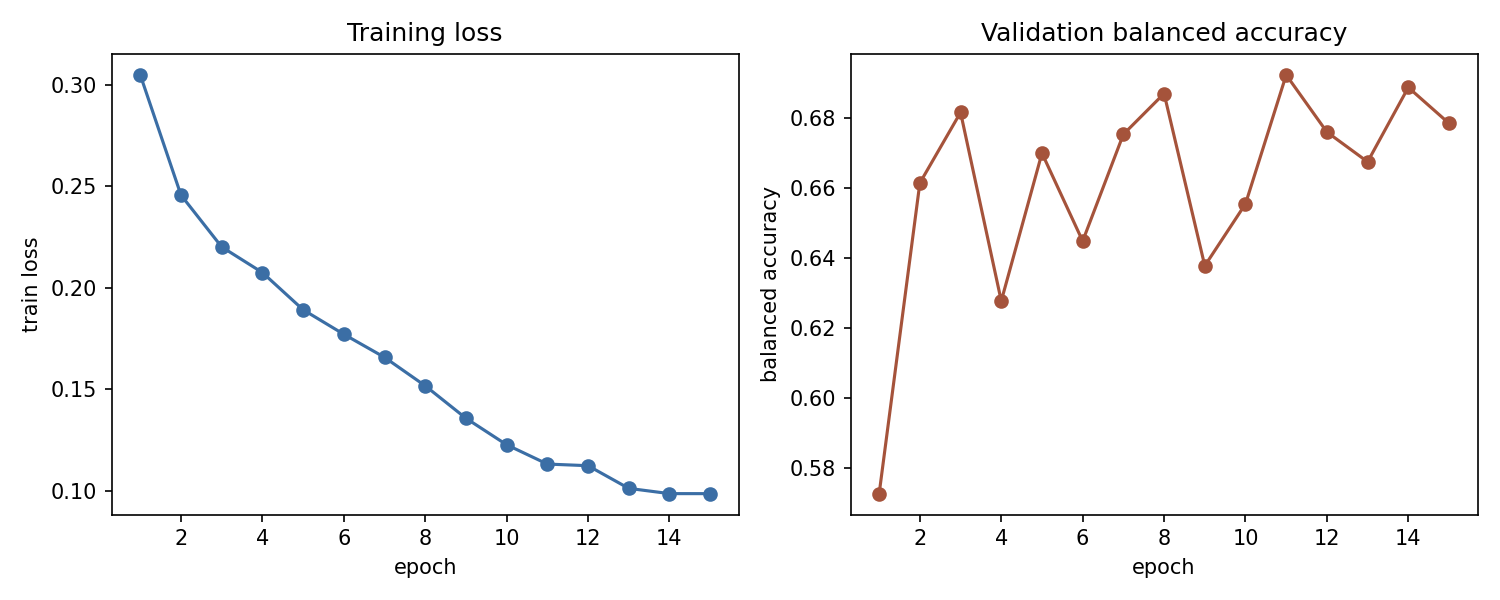
\includegraphics[width=\linewidth]{stage2_best_sensitivity_training_curves.png}
  \caption{Training loss and validation balanced accuracy for the median seed of ResNet-50 with the CE baseline. The model trains for 15 epochs and restores the best validation checkpoint.}
  \label{fig:training}
\end{figure}

\begin{figure}[t]
  \centering
  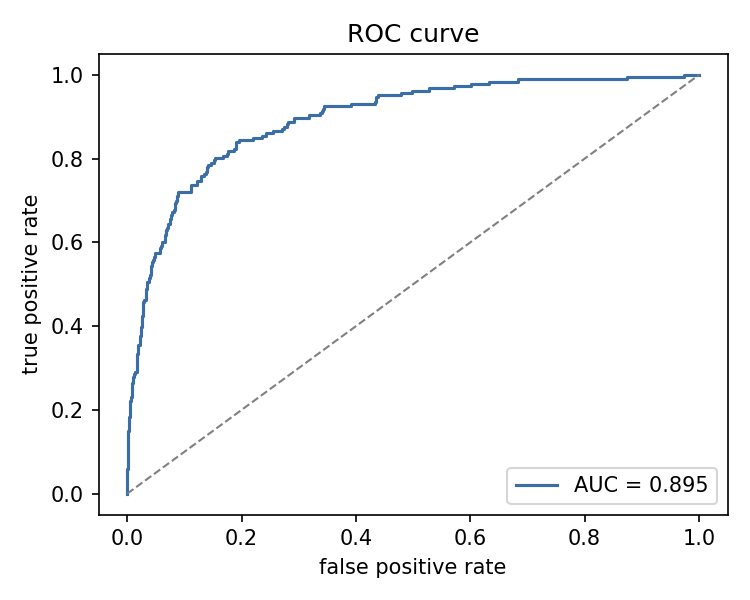
\includegraphics[width=0.72\linewidth]{stage2_best_sensitivity_roc_test.png}
  \caption{Test ROC curve for the median seed of ResNet-50 with the CE baseline. The operating threshold is selected on validation at 95\% specificity.}
  \label{fig:roc}
\end{figure}

\section{Discussion}

\subsection{Imbalance correction is architecture-dependent}

Focal loss with class-balanced sampling is not a neutral intervention. It helps the transformer and hurts both CNNs. A benchmark that applied the correction to one architecture and generalized the result would have reached the wrong conclusion about the others.

The effect has a plausible mechanism. Focal loss changes the gradient distribution, and class-balanced sampling changes the effective class prior. A transformer with weaker inductive bias may benefit from the harder examples and the reweighted prior, while a CNN with strong local features may overfit the minority samples or lose calibration. The experiment cannot separate those mechanisms. We report the effect as an empirical interaction, not a causal explanation.

\subsection{The ranking flip and the stable AUC}

The sensitivity ranking reverses, but the AUC ranking does not. EfficientNet-B0 remains first and ViT-S/16 remains last in both the baseline and corrected conditions. The reversal is therefore specific to the thresholded operating point.

This matters for how model comparisons are reported. A single threshold at 0.5, or a single sensitivity number, can make an architecture look better or worse depending on the correction. Reporting sensitivity at a fixed specificity, AUC, and calibration together gives a more complete picture. We leave a full calibration analysis to future work.

\subsection{The fairness signal}

The dark stratum has the lowest AUC and the highest false positive rate in all nine configurations. The direction is consistent even though the sample is small. The most likely interpretation is that the model's ranking quality degrades on darker images, which produces more false positives at the fixed specificity threshold.

The dark-stratum sensitivity is underpowered. Six melanoma cases cannot support a precise estimate, and the bootstrap intervals span the full range. We therefore treat the AUC and false positive rate as the more stable signals and the sensitivity estimate as inconclusive.

The light stratum is often harder than the medium stratum. This is consistent with a contrast effect: a pale lesion on pale skin has a lower boundary contrast, and the model may attend to the surrounding skin. Skin tone is not the only source of difficulty. Lesion contrast, hair, rulers, and illumination can all change the model's attention.

\subsection{The data bottleneck}

The external dermoscopic datasets with Fitzpatrick labels, HIBA and PROVe-AI, contain Fitzpatrick I-IV only. Pipsqueak, the only dermoscopic dark-skin set, has 16 core images. The clinical datasets with Fitzpatrick V-VI, such as DDI, SCIN, and PASSION, differ from HAM10000 in imaging modality.

This is the main obstacle to a strong dark-skin claim. This study can quantify the representation gap, report the consistent dark-stratum AUC and false-positive signal, and show the limitation of the available dermoscopic data. A precise dark-skin sensitivity estimate requires new dermoscopic data collection or a carefully controlled cross-modality study.

\subsection{What XAI adds}

The classification and fairness results describe what the model does. The XAI analysis tests whether it attends to the lesion or to the surrounding skin. If attribution mass outside the lesion is higher in the dark stratum and correlates with errors, attribution leakage becomes an early warning signal that can be measured before group-level sensitivity collapses. The protocol is defined in Section~3.9.

\subsection{Implications for model selection}

The choice of architecture depends on the correction. At the CE baseline, ResNet-50 has the highest sensitivity at 95\% specificity. Under focal loss with class-balanced sampling, ViT-S/16 is the best. A deployment decision that ignores the training condition can pick the wrong model.

For the fairness analysis, this means the evaluation should include the architecture-condition combinations, not a single global best model. The best model on aggregate sensitivity may not be the best model in the dark stratum, and the ranking may change again after the external validation.

\section{Limitations}

\begin{itemize}
  \item We use HAM10000 only. Cross-dataset generalization to PH2, BCN20000, or ISIC 2020 is not yet measured.
  \item The endpoint is binary melanoma versus all other diagnoses. Seven-class classification is a secondary experiment.
  \item Each condition uses three seeds. The seed standard deviation is reported, but more seeds would tighten the estimates.
  \item Stage 1 uses 160-pixel images and Stage 2 uses 224-pixel images. The two stages are not directly comparable.
  \item The fairness analysis uses an image-based lightness proxy, not clinical Fitzpatrick labels. The proxy is sensitive to illumination, color calibration, and lesion contrast.
  \item The dark stratum contains 43 test images and six melanomas. The sensitivity estimate is underpowered, and the dark-stratum results are a signal rather than a precise effect size.
  \item HIBA and PROVe-AI contain Fitzpatrick I-IV only. The clinical datasets with Fitzpatrick V-VI differ in imaging modality, so the dark-skin comparison is confounded.
  \item No clinician reader study was conducted, so the clinical relevance of the attribution maps is not yet validated with dermatologists.
  \item No deployed system, prospective validation, or regulatory analysis is included.
\end{itemize}

\section{Ethics and reproducibility}

All data are public, de-identified research datasets. HAM10000 and the ISIC archive are released for research use, and the external datasets are used under their respective licenses. The study involves no patient contact and no new data collection.

The system is a research prototype, not a diagnostic device. The results do not establish clinical utility.

The Fitzpatrick scale has known limitations: it is a coarse phototype scale, it does not capture the full range of skin tones, and it conflates pigmentation with UV response. We use it because the datasets and the fairness literature use it. The lightness strata are image-based measurements, not clinical labels.

The representation gap is a finding with an ethical consequence: the data needed to measure dark-skin performance are scarce. We report the small number of dark-skin dermoscopic images. Synthetic dark-skin images are not used to claim fairness improvements.

The code, configs, splits, per-sample predictions, and table generation scripts are released with the paper. The repository records the git commit, seed, device, and package versions for every run.

\section{Conclusion}

We benchmarked ResNet-50, EfficientNet-B0, and ViT-S/16 on HAM10000 under three pre-declared conditions. Focal loss with class-balanced sampling raised ViT-S/16 sensitivity by 8.2 points and lowered the two CNNs, which reversed the point-estimate ranking at 95\% specificity. The paired within-architecture intervals include zero, but the difference-in-differences between each CNN and the ViT excludes zero. The AUC ranking stayed stable, and focal loss roughly tripled expected calibration error. Calibration and threshold placement therefore help explain how the sensitivity ranking can change while the ranking quality of the scores does not. The direction of the effect still depends on the architecture.

The fairness analysis became more specific once the cutoff and the error type were separated. The dark stratum has a higher false positive rate at $L^*$ cutoffs of 55, 58, and 60, while the dark AUC deficit is present only at the strictest cutoff. Adjusted models show that darker skin is associated with more false positives and lighter skin with more false negatives, and that lesion-skin contrast moves both error types in opposite directions. Fairness in this setting is an error-type shift, not a single sensitivity gap.

The XAI analysis showed that all three architectures place less attribution inside the lesion on darker images. False negatives have lower attribution mass than false positives, which explains why the pooled mass-error correlation is weak. HIBA validation reproduced the CNN-transformer gap but showed a 16 to 18 point sensitivity drop, and HIBA contains no Fitzpatrick IV melanomas and no Fitzpatrick V-VI images.

The next steps are a clinical dark-skin evaluation with DDI or PASSION, two additional seeds for the six focal and CE cells, and a second attribution method. The clinical dataset is the main requirement for a precise Fitzpatrick V-VI claim. The additional seeds and the second attribution method would tighten the architecture interaction and test whether the error-type pattern is specific to Grad-CAM.


\bibliographystyle{plainnat}
\bibliography{references}

\end{document}
